\documentclass[twocolumn,onesided,9pt]{article}

\PassOptionsToPackage{table}{xcolor}

\usepackage{./Task32FlyerLatexStyle/Task32Flyer}
\usepackage{todonotes}

%% -----------------------------------
%% Document information
%% -----------------------------------
\def\pubdate{29 March 2021}
\title{WS16: Digitalisation of Wind Lidar}
\shorttitle{WS16: Digitalisation}
\doctype{IEA Wind Task 32 Workshop Minutes}
\DOI{10.5281/zenodo.xxxxxx}
\addbibresource{bibliography.bib}

%% -----------------------------------
%% Style modifications (doc specific)
%% -----------------------------------
% task 32 action box
\usepackage{tcolorbox}
\newtcolorbox{taskactions}[1][]
{
	every float=\centering,
	width=1.0\columnwidth,
	boxsep=0pt,
	left=3pt,
	right=3pt,
	top=3pt,
	colframe = Task32Blue2,
	#1,
}
% no indents
\setlength{\parindent}{0pt}
% long tables
\usepackage{supertabular}
% define figure and section references
\newcommand{\fref}[1]{Fig.~\ref{#1}}
\newcommand{\sref}[1]{\S~\ref{#1}}
% set the TOC depth
\setcounter{tocdepth}{2}
% reduce spacing in TOC
\usepackage[titles]{tocloft}
\setlength{\cftbeforesecskip}{3pt}
% authors
\newcommand{\orcid}[1]{\href{https://orcid.org/#1}{
\includegraphics[width=12pt]{graphics/ORCIDiD_icon128x128.png}}}
\usepackage{fontawesome}
\newcommand{\mailme}[1]{\href{mailto:#1}{\faicon{envelope-o}}}

%% ===================================
%:
%% Document starts
%% ===================================
\begin{document}

%% -----------------------------------
%% Title
%% -----------------------------------
\maketitle
\thispagestyle{cover}

%% -----------------------------------
%% Authors
%% -----------------------------------
\noindent\begin{minipage}{\columnwidth}
\textcolor{TextLightGrey}{Authors: Andrew Clifton~\orcid{0000-0001-9698-5083}~\mailme{clifton@ifb.uni-stuttgart.de}, %
Ines Würth~\orcid{},
David Schlipf~\orcid{}}
\end{minipage}
\vskip 6pt

%% -----------------------------------
%% Introductory text
%% -----------------------------------
{\Large\noindent%
What will digitalisation mean for wind lidar, and how can digitalised wind lidar be integrated with the digitalised wind energy business? 
}
\vskip 6pt

Wind energy and many other users of wind lidar are going digital, leveraging decades of developments in programming, more reliable communications, and the internet of things. This digital transformation will lead to new ways of working, new opportunities, and new business ideas. But it will also mean that wind lidar will change as well. Together, the wind energy industry and wind lidar will undergo digitalisation.

This workshop used a combination of presentations, group work, and discussions to explore what digitalisation might mean for wind lidar hardware, software, users, and stakeholders.

\tableofcontents

\section*{Disclaimer}
The presence of a person’s name or an organisation's name in this document (e.g., in the list of participants in Table \ref{tab:participants}) should not be taken to imply that that person or organisation agrees with any of the opinions set out here. Similarly, the use of any brand names or trade marks does not constitute an endorsement.

\section*{Attribution}
The workshop ran under modified Chatham House rules. Specifically, participants are free to use information from the discussion, but are not allowed to reveal who made any comment. Material presented by the three invited speakers (listed in “Digitalisation in Practice”) may be attributed.

\section{Agenda}

\begin{table}[!h]
 \centering
 % set up banded rows for the agenda and add lines to the columns
 \arrayrulecolor{Task32Blue2!15}
 \rowcolors{2}{Task32Blue2!5}{white}
 \begin{tabular}{@{}|p{0.125\columnwidth}|p{0.85\columnwidth}|@{}}
 \rowcolor{Task32Blue2} \textbf{Time} & \textbf{Activity} \\
 14:00 & Introduction \\
 14:20 & What is digitalisation?
  \begin{itemize}
        \item How the common lidar data format improved our data processing (Ines Würth, SWE)
        \item The Smart Lidar Concept - New Opportunities for the Lidar Community (David Schlipf)
	\item Modularising wind lidar (Andy Clifton)
    \end{itemize} \\
 15:00 & Working groups: user stories for different wind lidar scenarios\\
 16:00 & Sharing results\\
 16:45 & Close \\
 \end{tabular}
 \label{tab:agenda}
\end{table}


\section{Introduction: what is digitalisation?}

Wind lidar is an inherently digital measurement device in that the results of the measurement are digital signals (radial wind speed, wind vector, etc.). Similarly, wind turbines, wind plants, and the rest of the energy system infrastructure generate huge amounts of data. Digitalisation can be seen as the process whereby wind lidar data, wind energy system infrastructure data, and other data are used together to enable more reliable and more valuable energy. Together, they will enable the wind energy plant of tomorrow (Figure \ref{fig:digital_windplant}).

\begin{figure*}[!hbt]
    \centering
    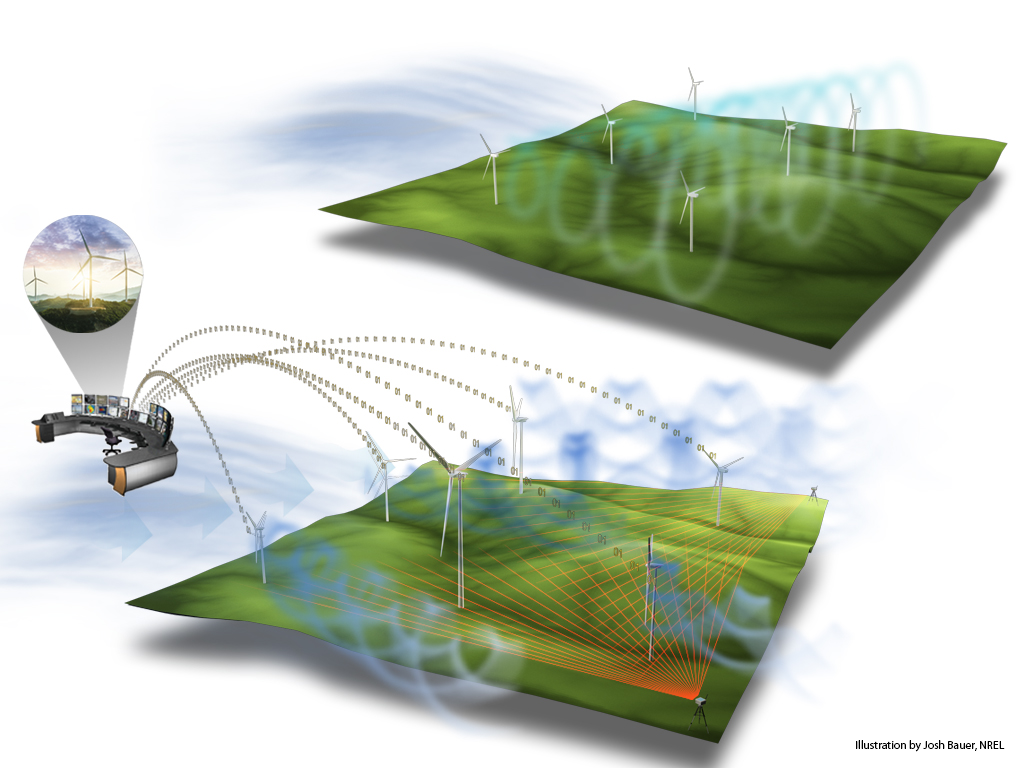
\includegraphics[width=0.85\textwidth]{figures/NRELTP-5000-68123-Fig4.png}
    \caption{Digitalisation of wind lidar and wind plants will enable the transition from the wind plant of today (top) to the networked wind plant of tomorrow (bottom). Figure courtesy Josh Bauer, NREL}
    \label{fig:digital_windplant}
\end{figure*}

However, it is difficult to know what digitalisation will involve until we have tried it. Therefore, this workshop set out to develop user stories for several different wind lidar usage scenarios. These are discussed in more detail in Section 3.
\section{Digitalisation in practice}

The workshop started with presentations by three groups that have all been exploring digitalisation of wind lidar.

\subsection{How the common lidar data format improved our data processing (Ines Würth, SWE)}

In 2018 DTU, Fraunhofer IEE and others published the report from their e-WindLidar project \citep{nikola_vasiljevic_2018_2478051} in which they introduced a common format for wind lidars. Up to now, lidars from different manufacturers spit out data in different formats using different variables. In Stuttgart we therefore developed different code for each lidar in order to process the data.

The common format brings only advantages: in Stuttgart we implemented it in our code and now only have one data processing routine for different lidar systems. Collaboration is facilitated because exchange of code and data is very easy. Interfaces where data is exchanged are clearly defined. Therefore we believe that the common data format is the basis for a digitized lidar infrastructure of the future.

The presentation can be found at \href{https://doi.org/10.5281/zenodo.4629675}{https://doi.org/10.5281/zenodo.4629675}.

\subsection{The Smart Lidar Concept - New Opportunities for the Lidar Community (David Schlipf)}

We believe that lidar systems will follow the general trend of technology by adapting to their environment and becoming more adjustable. Here, the “smart lidar” concept intends to provide a helpful framework. 

The smart lidar consists of a reprogrammable lidar device that can be modified or extended by “apps”. A first version of smart lidar was developed as part of the international research and development (R\&D) project between Flensburg University of Applied Sciences, MOLS and sowento. A commercial lidar has been modified to process third party algorithms which can be directly integrated in common simulation tools for wind turbines, which significantly simplifies the certification of lidar-assisted control applications. In future we anticipate that these apps can be provided by specialists, allowing lidar users and their customers to take advantage of the wide range of experience in the international wind lidar community. 

The presentation shows the main advantages, current advances, and new opportunities for various stakeholders in the lidar community. 

Further details can be found at \href{https://doi.org/10.5281/zenodo.4627168}{https://doi.org/10.5281/zenodo.4627168}. 

\subsection{Modular wind lidar (Andy Clifton, Task 32)}
Wind lidar are complex devices that are optimised for particular tasks. However, they often contain basically the same modules - power supply, communications, laser source, optics, scanner - that have different properties and capabilities depending on the task. In 2015 a group of Task 32 members came up with the “Open Lidar” concept for modular lidar \citep[Figure \ref{fig:modular_lidar} and ][]{clifton_2019_openlidar}, whereby different hardware and software would be combined for different applications. Modular wind lidar have been built in the past but are not commercially available at this time.

\begin{figure*}[!hbt]
    \centering
    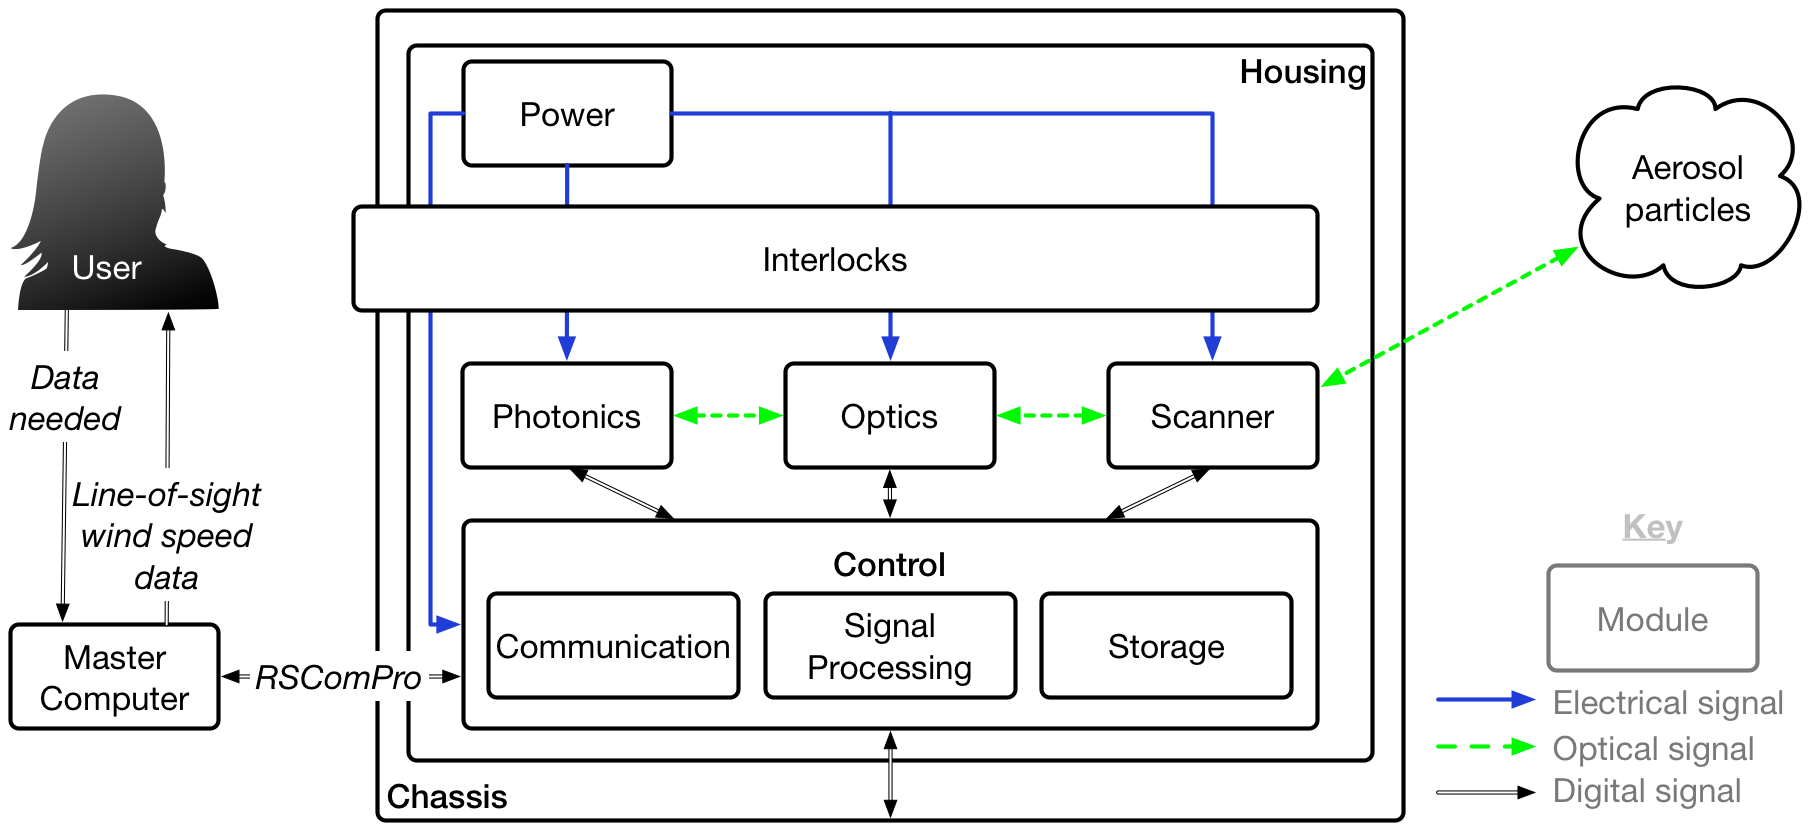
\includegraphics[width=0.85\textwidth]{figures/OpenLidarModules.png}
    \caption{The OpenLidar modular wind lidar architecture \cite{clifton_2019_openlidar}}
    \label{fig:modular_lidar}
\end{figure*}

The Open Lidar concept has since been applied as a generic, modular architecture for lidar, which is now documented in the Task 32 Wind Lidar Ontology. This generic architecture with clear definitions in turn enables the development of a “digital twin” for wind lidar - software representations of real-world hardware.

The first wind lidar digital twin - \emph{Qlunc}, designed to quantify the uncertainty of a lidar device - has just been released (DOI: \href{https://doi.org/10.5281/zenodo.4600881}{10.5281/zenodo.4600881}). Qlunc uses the open lidar architecture and defines uncertainty for the hardware components within each module. The uncertainties can then be combined to estimate the uncertainty of line-of-sight wind speed measurements and the total pointing and range uncertainty. This, in turn, can be used as an input to other tools, such as MOCALUM or YADDUM.

Together these tools offer the chance to effectively simulate wind lidar hardware for many different applications, and optimise them before building or deploying them.


\section{User stories for wind lidar digitalisation}

The workshop participants next split into small groups to create user stories for four different situations. These situations were proposed by the workshop organiser as representative of common situations:
\begin{itemize}
\item Wind resource assessment
\item Monitoring offshore wind turbines
\item Lidar for wind plant control
\item Lidar solution providers
\end{itemize}

The groups further defined the scenario and the current actors. They identified how these actors interact and what challenges they might face. They then considered how that scenario might change over the next three to five years, and how digitalisation might impact those scenarios. Finally, each group identified any potential “show-stoppers” and the highest priority activities to enable success. The results are summarised in the following subsections and are based on a template provided by the Workshop organiser. The results have not been edited and may include spelling errors or be unclear.

\begin{taskactions}
    Please report any corrections to the \href{mailto:ieawind.task32@ifb.uni-stuttgart.de}{Task 32 Operating Agent}.
\end{taskactions}
\subsection{Wind resource assessment}

This group considered a scenario in which a wind plant developer wants to deploy a wind lidar for a wind resource assessment campaign. The users include the lidar provider and several customers, including a data analyst, a data manager, and a project manager (Table \ref{tab:01_wra_now}).

This group felt that the biggest potential from digitalisation was the ability to feed back experience from measurement campaigns into the next campaign, and thus build up repeatable, high-quality wind resource assessment processes.

The group expected feedback to be enabled in the near future by the availability of more data and better data storage and retrieval. They expected the same actors still to be present in a wind resource assessment campaign, and with similar concerns as to today (Table \ref{tab:01_wra_future}).

The group identified the following things as being important to making this vision a reality:

\begin{enumerate}
\item
  \textbf{A data hub}: software and services to receive, manage and
  process data. This should be based on community standards and should
  be delivered by the lidar provider(s) and the community. It was noted
  that this should not be too complex, otherwise it might prevent
  adoption.
\item
  \textbf{Data standards}: clear standards for data and data products at
  different stages of the wind resource assessment process are required.
  They should be compatible with all sections of the wind energy
  industry. This should be delivered by the wind lidar and wind energy
  community. These were also seen as a priority.
\end{enumerate}

\subsection{Monitoring offshore wind turbines}

This group chose to explore the effects of digitalisation on forecasting for energy trading on 5- to 10-minute time scales.

They identified three actors involved in this at present:

\begin{itemize}
\item
  Alice, a wind farm operator. They currently record SCADA data and have no way to use this in their market. They are sometimes required to down-regulate their turbines by the grid operator.
\item
  Bob, a weather forecaster. They obtain satellite and other data to create a weather forecast
\item
  Chris, an energy trader. They trade energy from various sources.
\end{itemize}

Currently the three actors operate independently (Table \ref{tab:02_offshoreforecasting_now}). The group imagined a future state where the actors are able to interact and share data, enabling energy trading (Figure \ref{fig:02_offshoreforecasting_future}).

The group identified several things that would be needed to make this vision a reality:

\begin{enumerate}
\item
  \textbf{Good wind speed measurements from lidar}. The Lidar system
  with high range resolution would also need to provide a data flow to
  the forecaster. This should be provided by Lidar OEMs.
\item
  \textbf{Feedback from the market}. This would take the form of e.g., a
  command for regulation of the turbines. It was thought this would be
  provided by new companies.
\item
  \textbf{Improved forecasting method using lidar data}. Good forecasts
  are achieved with lidar data, so the data flow needs to be established
  between the wind farm operator and forecaster. This needs to be
  enabled by the forecasting company.
\item
  \textbf{Realtime data for energy trading and market flexibility} to enable real time energy trading. This needs to be done by Bob and the market.
\item
  \textbf{Standardized data formats}. We need standards for all data flows. This should be done by expert groups from IEA and IEC.
\end{enumerate}

The main potential barriers were seen as market regulations and the difficulty of establishing reliable, timely data flows.


\subsection{Wind plant control}

This group chose to explore the concept of ``Smart wind farms:
Nacelle-mounted lidar for wind farm optimisation''. This is currently an area of active research but very limited commercial adoption (Table \ref{tab:03_windPlantControl_now}).

The future user story was split into two phases (Table \ref{tab:03_windPlantControl_future}). The first phase takes place during the project execution:

\begin{enumerate}
\item
  Fred invests into a development project
\item
  Fred and Alice together provide communication network, database,
  processing power
\item
  Diane provides consultancy and advanced control algorithms
\item
  Bob connects lidar to the network and integrates lidar (reacts to
  commands)
\end{enumerate}

The second phase was after the project was complete:

\begin{enumerate}
\setcounter{enumi}{4}
\item
  All together publish their success stories
\item
  This will push others to do the same and can build up on the
  experience
\item
  Bob and Alice can improve their lidar / turbine to make them even
  smarter and can add more features.
\item
  Diane can develop better algorithms
\item
  Fred is happy and invests into more smart wind farms!
\end{enumerate}

Several things were identified as being required to make this vision a reality:

\begin{enumerate}
\item
  \textbf{Proof of concept}. First successful field testing needed. This
  could be done through a research project or JIP
\item
  \textbf{A common interface}. This would allow communication between
  lidars, turbines and the wind farm controller. This could be done by
  IEA Wind Task 32 + new wind farm flow control task
\item
  \textbf{Understanding of economic benefit}. How much is there to gain?
  How much are the investment/maintenance costs? This could be done by a
  research project, JIP, or in collaboration with IEA Wind Task 37.
\end{enumerate}

The main barriers to this happening were:

\begin{enumerate}
\item
  Data privacy / security issues
\item
  Unwillingness to share intellectual property
\item
  Lack of budget for development.
\end{enumerate}

The group felt that the priority for 2021 should be an economic model to convince the various players to step in.
\subsection{Lidar solutions provider}
The last group took the perspective of a lidar solutions provider (Alice), working with a customer (Chris) and a technician (Bob). Today, the lidar solutions provider and customer are not well connected (Table \ref{tab:04_lidarSolutionsProvider_now}).

The group expected moderate changes in the lidar market in the next five years (Table \ref{tab:04_lidarSolutionsProvider_future}). Specifically, they expected a shift to renting modular lidar that might be built with modules from several different hardware and software manufacturers, depending on the customer's needs.

The group identified several enabling steps that would be needed to make
this vision a reality:

\begin{enumerate}
\item
  \textbf{Modularity within lidar manufacturers}. Make lidar modules
  interchangeables. Software as well, monitoring,... This should be done
  by the manufacturers
\item
  \textbf{Standardization of lidar interfaces}. Provide standard data
  processing methods, interfaces. This should be done by IEA Task 32
\end{enumerate}

The major challenge to this was felt to be a lack of competition, i.e., the lack of pressure to change business practices.

The suggested priority for 2021 was the creation and use of a common and modular lidar interface for the input, output, and control of wind lidars.


\section{Summary}

The following section is a summary of the workshop and was prepared by the Operating Agent after the event.

\subsection{Priorities for 2021}

The following were seen as priorities to enable the digitalisation of wind lidar:

\begin{enumerate}
\item
  \textbf{Data standards} were required to enable wind lidar to be used for wind resource assessment, forecasting, wind plant controls, and to enable flexible, modular lidar.
\item
  \textbf{Data flows} to simplify data transfer from lidar devices to other devices and to users. This would be easier with data standards.
\item
  \textbf{A common and modular lidar interface} to enable data input and  output, and control of the wind lidar.
\item
  \textbf{Faster tools} that can be used as part of wind lidar-based   processes, e.g., for energy forecasting.
\item
  \textbf{Energy market flexibility} to allow new business models based on faster reaction times or greater flexibility, e.g., 5- to 10-minute-scale energy forecasting.
\item
  \textbf{Economic models} for different applications that demonstrate
  the economic case for investing in lidar.
\end{enumerate}

Other longer-term needs were identified for each scenario.

\subsection{Potential barriers to digitalisation}

\begin{enumerate}
\item  
  \textbf{Complexity}. Digitalisation is not easy and is a change from
  today's processes.
\item
  \textbf{Standards} that are too specific and incompatible.
\item
  \textbf{Market regulations} and the difficulty of establishing
  reliable, timely data flows.
\item
  \textbf{Data privacy and security issues}, including unwillingness to
  share intellectual property.
\item
  \textbf{Lack of budget for development}, limiting the scope for
  businesses to explore digitalisation.
\item
  \textbf{Lack of competition} to encourage change and new business
  models.
\end{enumerate}

\subsection{What can Task 32 do?}

This workshop showed that there are several things that IEA Wind Task 32 can do to support the digitalisation of wind lidar and it's integration into a digitalised wind energy business.

\begin{enumerate}
\item
  \textbf{Push data standards}. Some nascent data standards already exist,
  for example the e-WindLidar data format \cite{nikola_vasiljevic_2018_2478051} and \href{https://github.com/e-WindLidar/Lidaco}{the Lidaco data converters}. However, these only exist for line-of-sight data   and need to be extended to include processed wind lidar data. 
  \begin{taskactions}
    Task 32 will work with the developers and users of the e-WidLidar data format to extend it.
  \end{taskactions}
\item
  \textbf{Provide examples.} It is not always clear how digitalisation might work. Detailed examples for real use cases will help show the technology and processes that are required, and help understand the costs and benefits of digitalisation.
  \begin{taskactions}
    Task 32 will set up some examples of modular, multi-party collaborative data processing.
  \end{taskactions}
\item  
  \textbf{Encourage collaborative and open R\&D projects}. Task 32 members are
  already heavily involved with low-TRL projects that rely heavily on
  wind lidar data. The results from these projects need to be shared.
  And, where possible, the foundational tools that are developed should
  be shared with the rest of the community to help establish the
  infrastructure and market needed for digitalisation.
  \begin{taskactions}
    Task 32 will continue to provide a platform for the international wind lidar R\&D community to meet and exchange ideas and experience
  \end{taskactions}
\item
  \textbf{Collaborate with other IEA Wind Tasks}. Some Task 32 members
  are also involved with other relevant initiatives, for example IEA
  Wind Task 43 on the digitalisation of wind energy. 
  \begin{taskactions} 
  Task 32 will work with other stakeholder groups to explore how digitalised wind lidar would interface with
  other parts of the wind energy community.
  \end{taskactions}
\end{enumerate}

\section{Conclusions}
The results from this workshop are similar to those seen for studies of digitalisation in other areas of the wind energy industry. They include:

\begin{itemize}
    \item
    Digitalisation happens from the bottom up when users try to automate or reuse old processes, or to share them with colleagues. This can lead to competing, incompatible activities. We may be able to avoid this for wind lidar by leveraging common data formats at different parts of the process, for example the e-windLidar formats \citep{nikola_vasiljevic_2018_2478051}.
    \item 
    Digitalisation can also be top-down, for example by tasking internal teams or by buying in services. This can lead to an adoption problem, that can be avoided by working together with users to create the tools they need, and train them to use them.
    \item
    However it happens, digitalisation needs to be treated as an important (or even strategic) change that can heavily impact users.
    \item
    Like many businesses, the wind lidar business will become modular. Users will increasingly create their own processes based on a mixture of hardware and software tools. 
    \item 
    Service providers - hardware vendors, consultants, researchers - therefore need to work on simplifying the interfaces between their parts of the process.
    \item
    Standards will help with many aspects of digitalisation, as would data and app marketplaces.
    \item
    None of this will happen without management support and encouragement.
    \item 
    We need ways to talk about the costs and benefits of digitalisation.
\end{itemize}

\begin{taskactions}
IEA Wind Task 32 will be convening a working group to make progress on some of these issues. Please get in contact if you would like to take part.
\end{taskactions}

%% -----------------------------------
%% References
%% -----------------------------------
%\section*{References}
% bibliography
\label{sec:References}
\addcontentsline{toc}{section}{References}
{\small
	\printbibliography
}
\vspace*{\fill}

%% -----------------------------------
%% Outlined block of smaller text
%% -----------------------------------
\begin{tcolorbox}[width=1.0\columnwidth,
		boxsep=0pt,
		left=3pt,
		right=3pt,
		top=3pt,
		arc=0pt,
		boxrule=0.5pt,
		toprule=0.5pt,
		colback=white,
		coltext=TextGrey
	]
	{\footnotesize

		%% -----------------------------------
		%% IEA WIND AND TASK 32
		%% -----------------------------------
		
		\begin{tabular}{m{0.3\columnwidth}m{0.6\columnwidth}}
			\rowcolor{white}
			\multicolumn{2}{p{0.9\columnwidth}}{%
			This document was self published by IEA Wind Task 32.
			}\\
			% IEA Wind * DO NOT EDIT THIS TEXT *
			\rowcolor{white}
			
\includegraphics[height=2cm]{graphics/IEAWind_logo.jpg}  &
			The International Energy Agency is an autonomous organisation which works to ensure reliable, affordable and clean energy for its 30 member countries and beyond. The IEA Wind Technology Collaboration Programme supports the work of 38 independent, international groups of experts that enable governments and industries from around the world to lead programmes and projects on a wide range of energy technologies and related issues.%
			\\
			% Task 32 * DO NOT EDIT THIS TEXT *
			\rowcolor{white}
			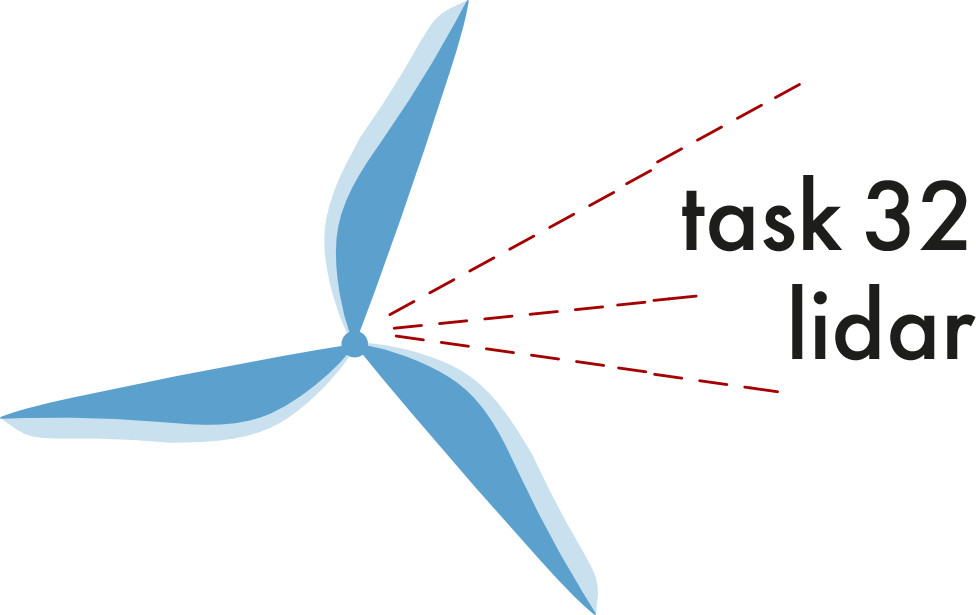
\includegraphics[height=1.5cm]{graphics/Task32_logo.jpg} &
			\href{https://community.ieawind.org/task32/home}{IEA Wind Task 32} exists to identify and mitigate the barriers to the deployment of wind lidar for wind energy applications.\\
			% authors, etc
			\rowcolor{white}
			\multicolumn{2}{p{0.9\columnwidth+2\tabcolsep}}{%
		%% -----------------------------------
		%% For more information
		%% -----------------------------------
		% N.B. do not add line breaks between the next items
		\textbf{For more information:} See the  \href{https://community.ieawind.org/task32/home}{Task 32 website}.
		%% -----------------------------------
		%% Authors
		%% -----------------------------------
		\textbf{Author team:} %
		Andrew Clifton (Task 32 Operating Agent, University of Stuttgart, Germany), %
		Ines Würth (SWE, University of Stuttgart, Germany), %		
		David Schlipf (Task 32 operating Agent, Flensburg University of Applied Sciences, Germany).
		%% -----------------------------------
		%% Reviewers
		%% -----------------------------------
		%\textbf{Reviewers:} %
		% first last (short affiliation), %
		% first last (short affiliation).
		%% -----------------------------------
		%% Images
		%% -----------------------------------
		\textbf{Images:}
		Banner, left to right: \href{https://unsplash.com/@alexkixa}{Alexandre Debiève on Unsplash}, \href{http://ifb.uni-stuttgart.de}{SWE U. Stuttgart}, \href{https://unsplash.com/@markusspiske}{Markus Spiske on Unsplash}.
	}\\
	\end{tabular}%

	}

	%% -----------------------------------
	%% End of highlighted block
	%% -----------------------------------
\end{tcolorbox}
\vspace*{\fill}

\clearpage
\begin{table*}[!h]
 \centering
 \caption{Actors in today's lidar-based wind resource assessments}
 % set up banded rows for the agenda and add lines to the columns
 \arrayrulecolor{Task32Blue2!15}
 \rowcolors{2}{Task32Blue2!5}{white}
 \begin{tabular}{@{}|p{0.125\textwidth}|p{0.185\textwidth}|p{0.185\textwidth}|p{0.185\textwidth}|p{0.185\textwidth}|@{}}
 \rowcolor{Task32Blue2} & \textbf{Alice} & \textbf{Bob} & \textbf{Darla} & \textbf{Cory} \\
They are: & 
    Lidar provider & 
    Data analyst & 
    Data manager & 
    Business / Project Manager \\
Their biggest problem is: & 
    Selling the lidar. 

    Deploying it on time &
    Configuring the lidar

    Uncertainty about metadata &
    Getting data into the organization and managing it. & 
    Knowing when to invest in using lidar. \\
Success for them is: & 
    Successful campaign with feedback from other campaigns &
    Good verification \& validation & 
    No issues during LiDAR data measurement &
    Clearer guideline on when investing in Lidar makes sense;

    Financing as planned \\
Problem statement & 
    \multicolumn{4}{p{0.74\textwidth+6\tabcolsep+3\arrayrulewidth}}{Need to get a ``good enough'' measurement for funding (enough data with sufficient uncertainty)} \\
\end{tabular}
\label{tab:01_wra_now}
\end{table*}
% note that the length of the multicolumn is managed by https://tex.stackexchange.com/a/204917

\begin{table*}[!h]
 \centering
 \caption{Actors in near-future lidar-based wind resource assessments}
 % set up banded rows for the agenda and add lines to the columns
 \arrayrulecolor{Task32Blue2!15}
 \rowcolors{2}{Task32Blue2!5}{white}
 \begin{tabular}{@{}|p{0.125\textwidth}|p{0.185\textwidth}|p{0.185\textwidth}|p{0.185\textwidth}|p{0.185\textwidth}|@{}}
 \rowcolor{Task32Blue2} & \textbf{Alice} & \textbf{Bob} & \textbf{Darla} & \textbf{Cory} \\
They are: & 
    Lidar provider & 
    Data analyst & 
    Data manager & 
    Business / Project Manager \\
Their biggest problem is: & 
    Selling the lidar. 
    
    Deploying it on time &
    Configuring the lidar; uncertainty about metadata & 
    Getting data into the organization and managing it. & 
    Knowing when to invest in using lidar \\
Success for them is: & 
    Successful campaign with feedback from other campaigns & 
    Good verification \& validation & 
    No issues during LiDAR data measurement & 
    Financing as planned / Clearer guideline on when investing in Lidar makes sense \\
Digitalisation helps by: & 
    Providing info & 
    Validation reports visual & 
    Smoother installation \& data management &
    Enabling Live queries of the project data and results \\
What problems are left? & 
    Maintaining standards & 
    Visual communication / reports & 
    Monitoring the lidar function, data storage, and security & 
    Uncertainty;

    ROI not clear 
\end{tabular}
\label{tab:01_wra_future}
\end{table*}
\clearpage
\begin{table*}[!h]
 \centering
 \caption{Actors in energy forecasting for offshore wind farms today}
 % set up banded rows for the agenda and add lines to the columns
 \arrayrulecolor{Task32Blue2!15}
 \rowcolors{2}{Task32Blue2!5}{white}
 \begin{tabular}{@{}|p{0.125\textwidth}|p{0.255\textwidth}|p{0.255\textwidth}|p{0.255\textwidth}|@{}}
 \rowcolor{Task32Blue2} & \textbf{Alice} & \textbf{Bob} & \textbf{Chris}  \\
They are: & 
    Wind farm operator & 
    Forecaster & 
    Energy trader \\
Their biggest problem is: & 
    Unknown wind conditions in the future & 
    No data & 
    If they cannot deliver sold energy \\
Success for them is: & 
    Wants to sell her energy & 
    Having low uncertainty forecast & 
    Highest revenue \\
Problem statement: & 
    \multicolumn{3}{|p{0.765\textwidth+4\tabcolsep+2\arrayrulewidth}|}{We need the best wind data to produce a low-uncertainty energy yield forecast}\\
\end{tabular}
\label{tab:02_offshoreforecasting_now}
\end{table*}


\begin{figure*}
    \centering
    \fbox{
    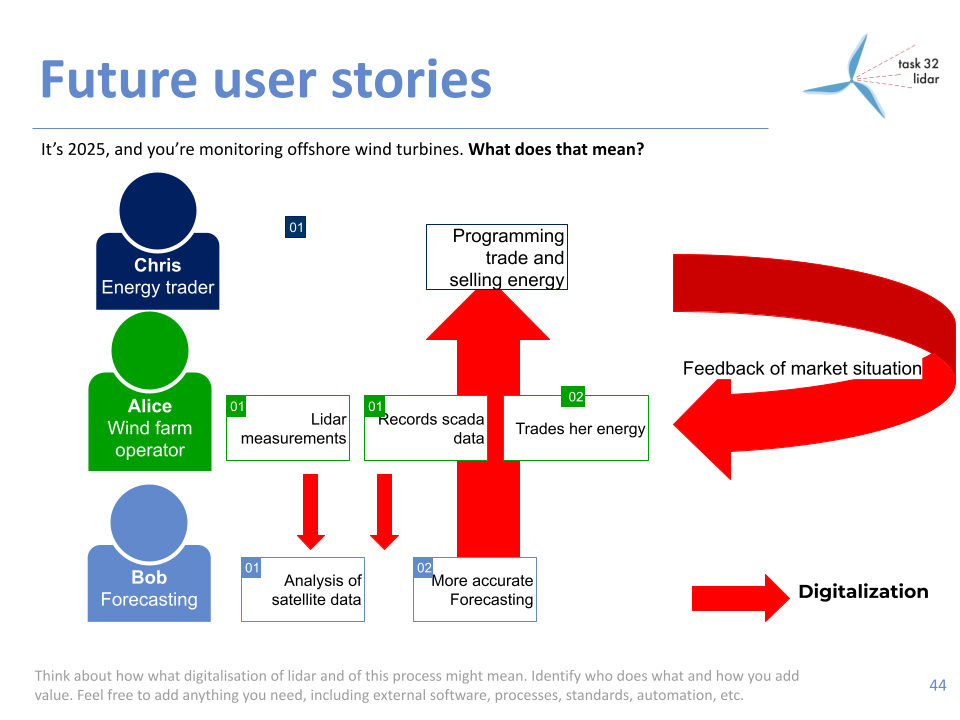
\includegraphics[width=0.85\textwidth]{figures/02_offshoreforecasting.png}
    }
    \caption{A vision for future energy trading for offshore wind}
    \label{fig:02_offshoreforecasting_future}
\end{figure*}

\clearpage
\begin{table*}[!h]
    \centering
    \caption{Actors in today's lidar-enabled wind plant control}
    % set up banded rows for the agenda and add lines to the columns
    \arrayrulecolor{Task32Blue2!15}
    \rowcolors{2}{Task32Blue2!5}{white}
    \begin{tabular}{@{}|p{0.125\textwidth}|p{0.185\textwidth}|p{0.185\textwidth}|p{0.185\textwidth}|p{0.185\textwidth}|@{}}
    \rowcolor{Task32Blue2} & 
        Alice &
        Bob & 
        Fred & 
        Diane \\
They are: & 
    Turbine OEM & 
    Lidar OEM & 
    Farm owner / operator &
    Independent analyst / engineer \\
Their biggest problem is: &
    Maintaining customer trust (customer already wants turbine), but OEM has to ensure performance. 
    
    Ensuring equipment operates in the best way.
    
    Need to avoid bad publicity as the turbine OEM is often blamed first. & 
    Ensuring durability of equipment.

    Clear view of what the data is being used for and how this can benefit. &
    Access to turbine controller to allow lidar to optimise farm for them.
    
    O\&M schedule increase turbine downtime (perhaps). &     
    No access to data.
    
    Standardised data format could cause problems for them also. \\
Success for them is: & 
    Better understanding of turbines and performance in non-benign conditions. 
    
    Better experience for end user. 
    
    Critical failure avoidance. &
    Ensuring durability, performance, acceptance and value proposition of systems. & 
    Optimised asset(s) (higher AEP, lifetime extension, lower O\&M, reduced LCoE). &
    Credible service development, success of data science application. \\
Problem statement: &
\multicolumn{4}{p{0.74\textwidth+6\tabcolsep+3\arrayrulewidth}}{No real solution for data to be compiled and interpreted in an easy and efficient way to make the most of this solution.

	No one wants to cover the overall development costs for proof on concept.

	Data security.

	Infrastructure for data sharing/communication across parts of the site} \\
\end{tabular}
\label{tab:03_windPlantControl_now}
\end{table*}


\begin{table*}[!h]
    \centering
    \caption{Actors in future lidar-enabled wind plant control}
    % set up banded rows for the agenda and add lines to the columns
    \arrayrulecolor{Task32Blue2!15}
    \rowcolors{2}{Task32Blue2!5}{white}
    \begin{tabular}{@{}|p{0.125\textwidth}|p{0.185\textwidth}|p{0.185\textwidth}|p{0.185\textwidth}|p{0.185\textwidth}|@{}}
    \rowcolor{Task32Blue2} & 
        Alice &
        Bob & 
        Fred & 
        Diane \\
They are: & 
    Turbine OEM & 
    Lidar OEM & 
    Farm owner / operator &
    Independent analyst / engineer \\
Digitalisation helps by: & 
    Certification.
    
    More realistic simulations.
    
    More awareness of their turbines.
    
    Strengthened relation with customer.&
    Make lidar systems more

    - helpful

    - accepted

    - adjustable

    - adaptive &
    Having more control of the farm output.
    
    Having more flexibility in the way it which the farm can be operated.

    AEP/load balancing. & 
    Accessing large quantities of data and develop apps/tools to bundle them and process them into more valuable refined product. \\

    Any problems left? & -- & -- & -- & -- \\
\end{tabular}
\label{tab:03_windPlantControl_future}
\end{table*}

\clearpage

\begin{table*}[!h]
    \centering
    \caption{Actors in providing lidars today}
    % set up banded rows for the agenda and add lines to the columns
    \arrayrulecolor{Task32Blue2!15}
    \rowcolors{2}{Task32Blue2!5}{white}
    \begin{tabular}{@{}|p{0.125\textwidth}|p{0.255\textwidth}|p{0.255\textwidth}|p{0.255\textwidth}|@{}}
    \rowcolor{Task32Blue2} & Alice & & Chris \\
    They are: &
        Provider &
        &
        Customer \\
    Their biggest problem is: &
        Provide the right device to Lisa & 
        &
        Can't correctly interpret the data or get out needed data \\
    Success for them is: &
        Provide the right device for the right price &
        &
    Long term use of the device \\
    Problem statement: &
        \multicolumn{3}{|p{0.765\textwidth+4\tabcolsep+2\arrayrulewidth}|}{The connection between the provider and customer is missing}
\end{tabular}
\label{tab:04_lidarSolutionsProvider_now}
\end{table*}

\begin{figure*}
    \centering
    \fbox{
    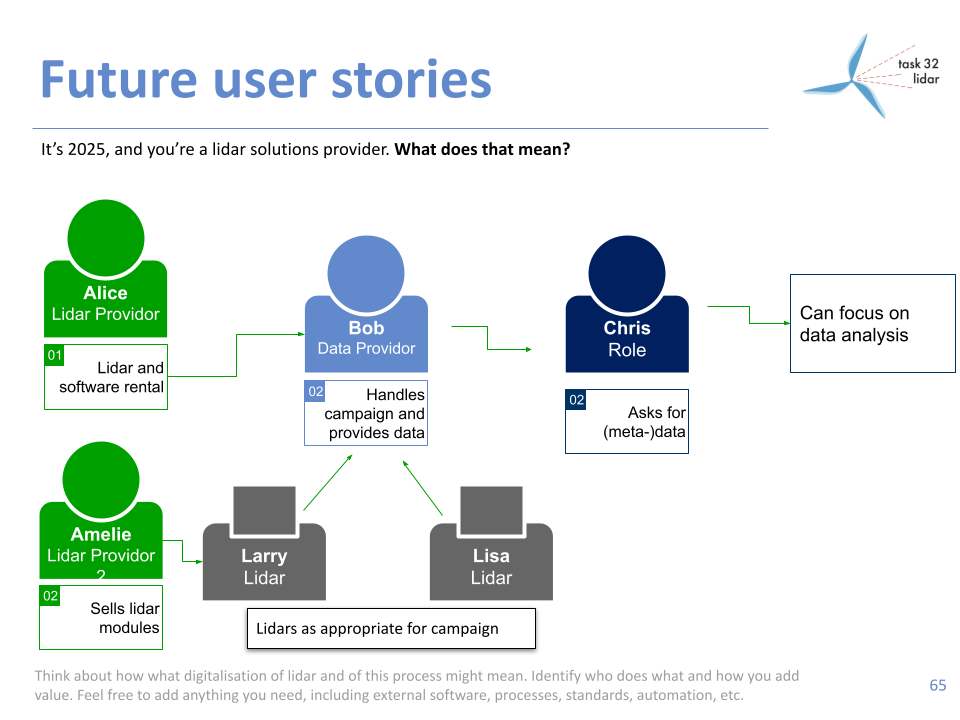
\includegraphics[width=0.85\textwidth]{figures/04_lidarSolutionsProvider.png}
    }
    \caption{Actors in a future lidar market}
    \label{fig:02_offshoreforecasting_future}
\end{figure*}


\begin{table*}[!h]
    \centering
    \caption{Actors in providing lidars in the future}
    % set up banded rows for the agenda and add lines to the columns
    \arrayrulecolor{Task32Blue2!15}
    \rowcolors{2}{Task32Blue2!5}{white}
    \begin{tabular}{@{}|p{0.125\textwidth}|p{0.255\textwidth}|p{0.255\textwidth}|p{0.255\textwidth}|@{}}
    \rowcolor{Task32Blue2} & Alice & Bob & Chris \\
    They are... & 
        Lidar Provider & Data Provider & Customer \\
    Their biggest problem is: &
        Selling less lidars because they will be rented &
        Handling different lidar data & 
        Need to define clearly what type of data is needed \\
    Success for them is: & 
        Operating a fleet of lidars for customer & 
        Get a common method to analyze data from different lidars & 
        More time for data analysis \\
    Digitalisation helps by: &
        Managing and monitoring lidars, gaining knowledge &
        Compare data

        Finding the most suitable lidar depending on site characteristics/ino want to get out &
        Providing insights and solutions faster. No need for handling lidar by additional staff. \\
    Any problems left? & 
        Have to stand out among other lidar providers.

        Modularity of software and hardware & 
        Defining tasks of data provider, common data and interface formats. 
    
        Managing lots of lidars effectively. &
        Who owns the data (only licence for usage or ownership)?
\end{tabular}
\label{tab:04_lidarSolutionsProvider_future}
\end{table*}

\clearpage

\begin{table*}
    \centering
    \caption{Participants}
    % set up banded rows for the agenda and add lines to the columns
    \arrayrulecolor{Task32Blue2!15}
    \rowcolors{2}{Task32Blue2!5}{white}
    \begin{tabular}{@{}|p{0.2\textwidth}|p{0.5\textwidth}|p{0.15\textwidth}|@{}}
    \rowcolor{Task32Blue2} Name & Affiliation & Country \\
	Alexandra Arntsen & NRG Systems & USA \\
	Amit Bohara & Altosphere Analytics & USA \\
	Andy Clifton & Operating Agent

(Stuttgart Wind Energy, University of Stuttgart) & Germany \\
	Peter Clive & Black and Veatch & UK \\
	Francisco Costa & Stuttgart Wind Energy, University of Stuttgart &
Germany \\
	Wei Fu & Danish Technical University & Denmark \\
	Ashim Giyanani & Fraunhofer IWES & Germany \\
	Sven-Erik Gryning & Danish Technical University & Denmark \\
Feng Guo & DTU Wind Energy & Denmark \\
Martin Hofs\"aß & Stuttgart Wind Energy, University of Stuttgart &
Germany \\
	Poul Hummelshøj & METEK Nordic ApS & Denmark \\
	Gyeongil Kwak & Engie & Germany \\
	Riaan Meyer & Geosun & South Africa \\
	Priscilla Orozco & UL & Germany \\
	Marcos Ortensi & University of Oldenburg & Germany \\
	Steffen Raach &
		sowento GmbH & Germany \\
	CarloAlberto Ratti & Vestas & Portugal \\
	David Schlipf & 
		Operating Agent

		(Flensburg University of Applied Sciences) & Germany \\
	Juan Jose Trujillo & UL & Germany \\
	Krithika v &
		National Institute of Wind Energy & India \\
	Maayen Wigger & Center for Solar Energy and Hydrogen Research Baden-Württemberg (ZSW) & Germany \\
	Ines Wuerth & Stuttgart Wind Energy, University of Stuttgart & Germany \\
	Scott Wylie & ZX Lidars & UK \\
	\end{tabular}
\label{tab:participants}
\end{table*}


\end{document}
